\UseRawInputEncoding
\documentclass[a4paper, 14pt]{extarticle}

% Поля
%--------------------------------------
\usepackage{geometry}
\geometry{a4paper,tmargin=2cm,bmargin=2cm,lmargin=3cm,rmargin=1cm}
%--------------------------------------


%Russian-specific packages
%--------------------------------------
\usepackage[T2A]{fontenc}
\usepackage[utf8]{inputenc} 
\usepackage[english, main=russian]{babel}
\usepackage{cmap}
%--------------------------------------

\usepackage{textcomp}

% Красная строка
%--------------------------------------
\usepackage{indentfirst}               
%--------------------------------------             


%Graphics
%--------------------------------------
\usepackage{graphicx}
\graphicspath{ {./images/} }
\usepackage{wrapfig}
%--------------------------------------

% Полуторный интервал
%--------------------------------------
\linespread{1.3}                    
%--------------------------------------

%Выравнивание и переносы
%--------------------------------------
% Избавляемся от переполнений
\sloppy
% Запрещаем разрыв страницы после первой строки абзаца
\clubpenalty=10000
% Запрещаем разрыв страницы после последней строки абзаца
\widowpenalty=10000
%--------------------------------------

%Списки
\usepackage{enumitem}

%Подписи
\usepackage{caption} 

%Гиперссылки
\usepackage{hyperref}

\hypersetup {
	unicode=true
}

%Рисунки
%--------------------------------------
\DeclareCaptionLabelSeparator*{emdash}{~--- }
\captionsetup[figure]{labelsep=emdash,font=onehalfspacing,position=bottom}
%--------------------------------------

\usepackage{tempora}
\usepackage{amsmath}
\usepackage[dvipsnames]{xcolor}
\usepackage{listings}
\lstset{
  belowcaptionskip=1\baselineskip,
  breaklines=true,
  frame=L,
  xleftmargin=\parindent,
  language=Java,
  showstringspaces=false,
  basicstyle=\footnotesize\ttfamily,
  keywordstyle=\bfseries\color{blue},
  commentstyle=\itshape\color{purple},
  identifierstyle=\color{black},
  stringstyle=\color{red},
  numbers=left,           
  numberstyle=\tiny\color{gray}, 
  numbersep=10pt,      
  % ------------------------------
}

%--------------------------------------
%			НАЧАЛО ДОКУМЕНТА
%--------------------------------------

\begin{document}

%--------------------------------------
%			ТИТУЛЬНЫЙ ЛИСТ
%--------------------------------------
\begin{titlepage}
\thispagestyle{empty}
\newpage


%Шапка титульного листа
%--------------------------------------
\vspace*{-60pt}
\hspace{-65pt}
\begin{minipage}{0.3\textwidth}
\hspace*{-20pt}\centering

\includegraphics[width=\textwidth]{emblem}
\end{minipage}
\begin{minipage}{0.67\textwidth}\small \textbf{
\vspace*{-0.7ex}
\hspace*{-6pt}\centerline{Министерство науки и высшего образования Российской Федерации}
\vspace*{-0.7ex}
\centerline{Федеральное государственное бюджетное образовательное учреждение }
\vspace*{-0.7ex}
\centerline{высшего образования}
\vspace*{-0.7ex}
\centerline{<<Московский государственный технический университет}
\vspace*{-0.7ex}
\centerline{имени Н.Э. Баумана}
\vspace*{-0.7ex}
\centerline{(национальный исследовательский университет)>>}
\vspace*{-0.7ex}
\centerline{(МГТУ им. Н.Э. Баумана)}}
\end{minipage}
%--------------------------------------

%Полосы
%--------------------------------------
\vspace{-25pt}
\hspace{-35pt}\rule{\textwidth}{2.3pt}

\vspace*{-20.3pt}
\hspace{-35pt}\rule{\textwidth}{0.4pt}
%--------------------------------------

\vspace{1.5ex}
\hspace{-35pt} \noindent \small ФАКУЛЬТЕТ\hspace{80pt} <<Информатика и системы управления>>

\vspace*{-16pt}
\hspace{47pt}\rule{0.83\textwidth}{0.4pt}

\vspace{0.5ex}
\hspace{-35pt} \noindent \small КАФЕДРА\hspace{50pt} <<Теоретическая информатика и компьютерные технологии>>

\vspace*{-16pt}
\hspace{30pt}\rule{0.866\textwidth}{0.4pt}
  
\vspace{11em}

\begin{center}
\Large {\bf Летучка № 5} \\ 
\large {\bf по курсу <<Языки и методы программирования>>} \\ 
\large <<Консольный сабскрайбер и ридер для MQTT-брокера>>
\end{center}\normalsize

\vspace{8em}


\begin{flushright}
  {Студент группы ИУ9-21Б Воронков А. С.\hspace*{15pt} \\
  \vspace{2ex}
  Преподаватель Посевин Д. П.\hspace*{15pt}}
\end{flushright}

\bigskip

\vfill
 

\begin{center}
\textsl{Москва 2026}
\end{center}
\end{titlepage}
%--------------------------------------
%		КОНЕЦ ТИТУЛЬНОГО ЛИСТА
%--------------------------------------

\renewcommand{\ttdefault}{pcr}

\setlength{\tabcolsep}{3pt}
\newpage
\setcounter{page}{2}

\section{Задание}
Написать простую консольную читалку и писалку
\section{Практическая реализация}
Код файла PublisherOld.java
\begin{lstlisting}
import org.eclipse.paho.client.mqttv3.*;
import java.util.Scanner;

public class PublisherOld {
    public static void main(String[] args) {
        String broker = "tcp://broker.emqx.io:1883";
        String clientId = "voronkov_java_pub";
        String topic = "IU/9/voronkov";

        try {
            MqttClient client = new MqttClient(broker, clientId);
            MqttConnectOptions opts = new MqttConnectOptions();
            opts.setCleanSession(true);

            System.out.println("Connecting to broker...");
            client.connect(opts);
            System.out.println("Connected!");

            Scanner scanner = new Scanner(System.in);
            while (true) {
                String payload = scanner.nextLine();
                MqttMessage message = new MqttMessage(payload.getBytes());
                client.publish(topic, message);
                System.out.println("ok");
            }

        } catch (MqttException e) {
            System.err.println("Ошибка MQTT: " + e.getMessage());
            e.printStackTrace();
        }
    }
}
\end{lstlisting}
\per
Код файла SubscriberOld.java
\begin{lstlisting}
import org.eclipse.paho.client.mqttv3.*;

public class SubscriberOld {

    public static void main(String[] args) {
        String broker = "tcp://broker.emqx.io:1883";
        String topic = "IU/9/voronkov";
        String clientId = "voronkov_subscriber";
        try {
            MqttClient client = new MqttClient(broker, clientId);
            MqttConnectOptions opts = new MqttConnectOptions();

            client.setCallback(new MqttCallback() {
                public void messageArrived(String topic, MqttMessage message) throws Exception {
                    String mes = new String(message.getPayload());
                    System.out.println("message content: " + mes);
                }

                public void connectionLost(Throwable cause) {
                    System.out.println("connectionLost: " + cause.getMessage());
                }

                public void deliveryComplete(IMqttDeliveryToken token) {
                    System.out.println("deliveryComplete: " + token.isComplete());
                }
            });

            System.out.println("Connecting to broker...");
            client.connect(opts);

            client.subscribe(topic);
            System.out.println("waiting");
        } catch (MqttException e) {
            System.err.println("Ошибка MQTT: " + e.getMessage());
            e.printStackTrace();
        }
    }
}
\end{lstlisting}

\begin{center}
    \nopagebreak
    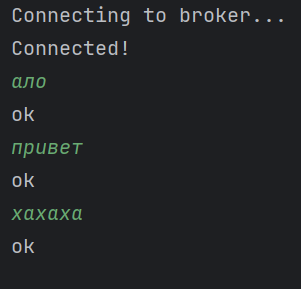
\includegraphics[width=0.85\textwidth]{let5_1}
    \captionsetup{justification=centering}
    \captionof{figure}{Визуализация работы писалки}

    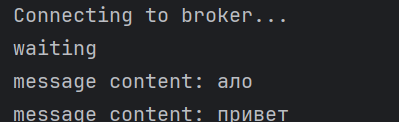
\includegraphics[width=0.85\textwidth]{let5_2}
    \captionsetup{justification=centering}
    \captionof{figure}{Визуализация работы читалки}
\end{center}

\section{Вывод}
В данной лабораторной работе были получены навыки работы с протоколом MQTT. Была написана своя читалка и писалка
\end{document}